\chapter{\label{ch:3-protodune}The ProtoDUNE--SP Experiment} 

\minitoc

%%%%%%%%%%%%%%%%%%%%%%%%%%%%%%%%%%%%%%%%%%%%%%%%%%%%%%%%%%%%%%%%%%%%%%%%%%%%%%%%
% From COS
%
% This chapter will discuss the ProtoDUNE--SP experiment and it's role in the
% development of the proposed DUNE experiment. The LArTPC technology will be
% detailed in the general case and then the specifics of the ProtoDUNE--SP
% detector will be given. Details of the major particle fluxes in ProtoDUNE--SP
% will be outlined, along with a discussion of the simulation and reconstruction
% of each flux. Finally, as my main contribution to detector operations during
% data taking was developing for the ProtoDUNE--SP online monitoring system, this
% will be discussed in more depth. 
% 
% The work for the online monitoring subsection has been completed as part of my
% duties as an on--site expert at CERN. I expect to be able to complete the rest
% of the work by the end of December 2019 alongside the other analysis work.
%%%%%%%%%%%%%%%%%%%%%%%%%%%%%%%%%%%%%%%%%%%%%%%%%%%%%%%%%%%%%%%%%%%%%%%%%%%%%%%%

% TODO: figure of experiment? 
% TODO: introductory chapter
\protodune{} is one of two prototypes for the DUNE far detector modules that has
been operating at the Neutrino Platform at CERN since the summer of 2018. The
experiment collected data from a charged particle beam for approximately 3 
months before Long Shutdown 2 of the Large Hadron Collider. Since then a 
programme of cosmic ray data collection has been ongoing.

% TODO: Chapter outline
This chapter will outline the technical details of the \protodune{} experiment.
Section \ref{sec:pdsp_dune} will outline the role of \protodune{} in the context
of the DUNE experiment. This will be followed by a discussion of the main
elements of the experiment, the \protodune{} detector systems and the H4
beam line, in Sections \ref{sec:pdsp_detector} and \ref{sec:h4} respectively.
The high event rate in \protodune{} is dominated by a high flux of comsic rays
which will be discussed in Section \ref{sec:pdsp_cosmic}. Section
\ref{sec:pdsp_sim_reco} will then discuss the simulation and reconstruction of 
\protodune{} data. Finally Section \ref{sec:pdsp_om} will cover details of the 
online monitoring system in \protodune{}; as the primary developer and expert 
on the \protodune{} online monitoring system during my time at CERN, the 
development and maintenance of this system represent a significant body of 
work over 12 months.  

\section{The DUNE Experiment and \protodune{}} \label{sec:pdsp_dune}

\begin{figure}

	\centering

	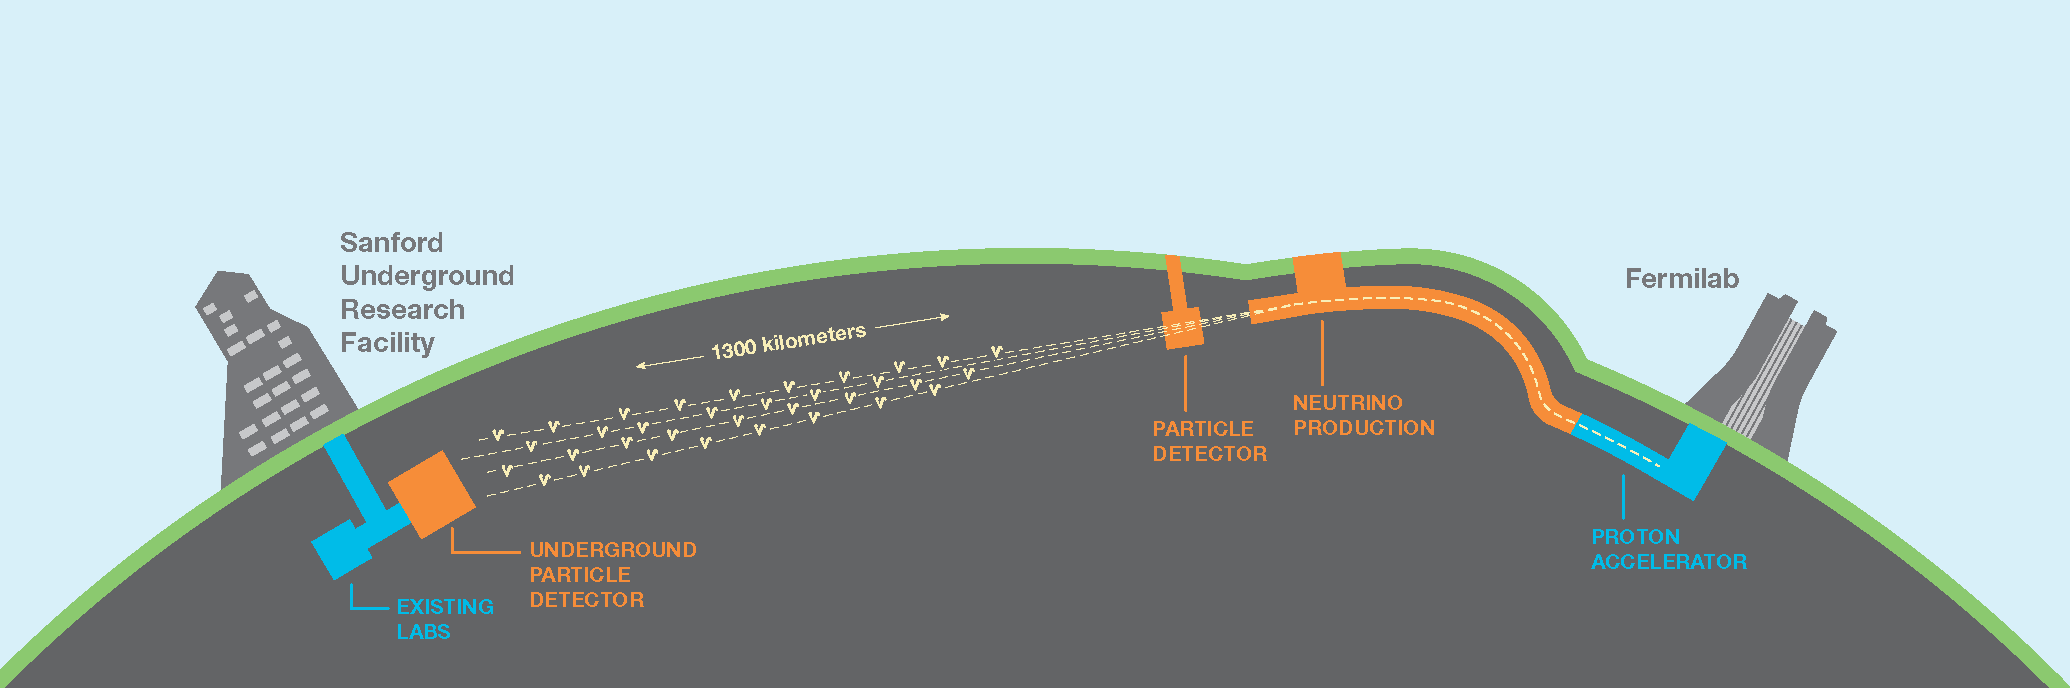
\includegraphics[width=\textwidth]{figures/dune_baseline.png}

	\caption
	[The Deep Underground Neutrino Experiment.]
	{The Deep Underground Neutrino Experiment. Figure from \cite{TODO}.}

	\label{fig:dune_baseline}

\end{figure}

The DUNE experiment will be a next generation neutrino physics and nucleon decay
experiment consisting of three principal components; an intense broad band 
neutrino beam and precise near detector based at the Fermilab National 
Accelerator Laboratory near Chicago, and a far detector at Sanford Underground 
Research Facility in South Dakota, approximately 1300 km away from the 
neutrino source, as demonstrated in Figure \ref{fig:dune_baseline}. The DUNE 
experiment identifies three primary scientific goals 
\cite{Abi:2020evt}:
\begin{itemize}
	\item Perform a comprehensive programme of neutrino oscillation measurements
	including measurements of \dcp{}, neutrino mass ordering, and the
	$\theta_{23}$ octant.
	\item Search for proton decay in several decay modes.
	\item Measure $\nu_e$ from a core--collapse supernova if one occurs within our
	galaxy during the lifetime of the experiment.
\end{itemize}
In addition, the experiment hopes to fulfill a significant programme of
secondary science goals:
\begin{itemize}
	\item Other accelerator based neutrino physics, such as non--standard
	interactions, sterile neutrinos, and CPT violation.
	\item Measurements of neutrino properties using atmospheric neutrinos.
	\item Dark matter searches in both the near and far detectors.
	\item A programme of neutrino interaction physics studies in the DUNE near
	detector.
\end{itemize}

To achieve these goals DUNE has opted to base the near and far detector designs
on the liquid argon time projection chamber (LArTPC) technology. The DUNE
far detector will consist of four LArTPC detectors each with 10 kt of active
liquid argon mass. This technology will have never before been used on this
scale, and therefore, there has been a significant programme of LArTPC research
and development ongoing to validate and characterise the performance of the 
technology for DUNE. 

\subsection{Liquid Argon Time Projection Chambers}
A LArTPC consists of a large volume of highly--purified liquid argon immersed in
an electric field. Charged particles traversing the liquid argon produce two
primary energy depositions, a trail of ionisation electrons along their path,
and prompt ultra--violet scintillation photons. After deposition the ionisation
electrons drift in the electric field toward the charge readout plane where they
induce electrical signals. Liquid argon is transparent to its own scintillation
light and therefore the scintillation photons can travel through the argon to be
collected in a photon detection system.The LArTPC detection principal is 
illustrated in Figure \ref{fig:lartpc}. 

\begin{figure}

	\centering

	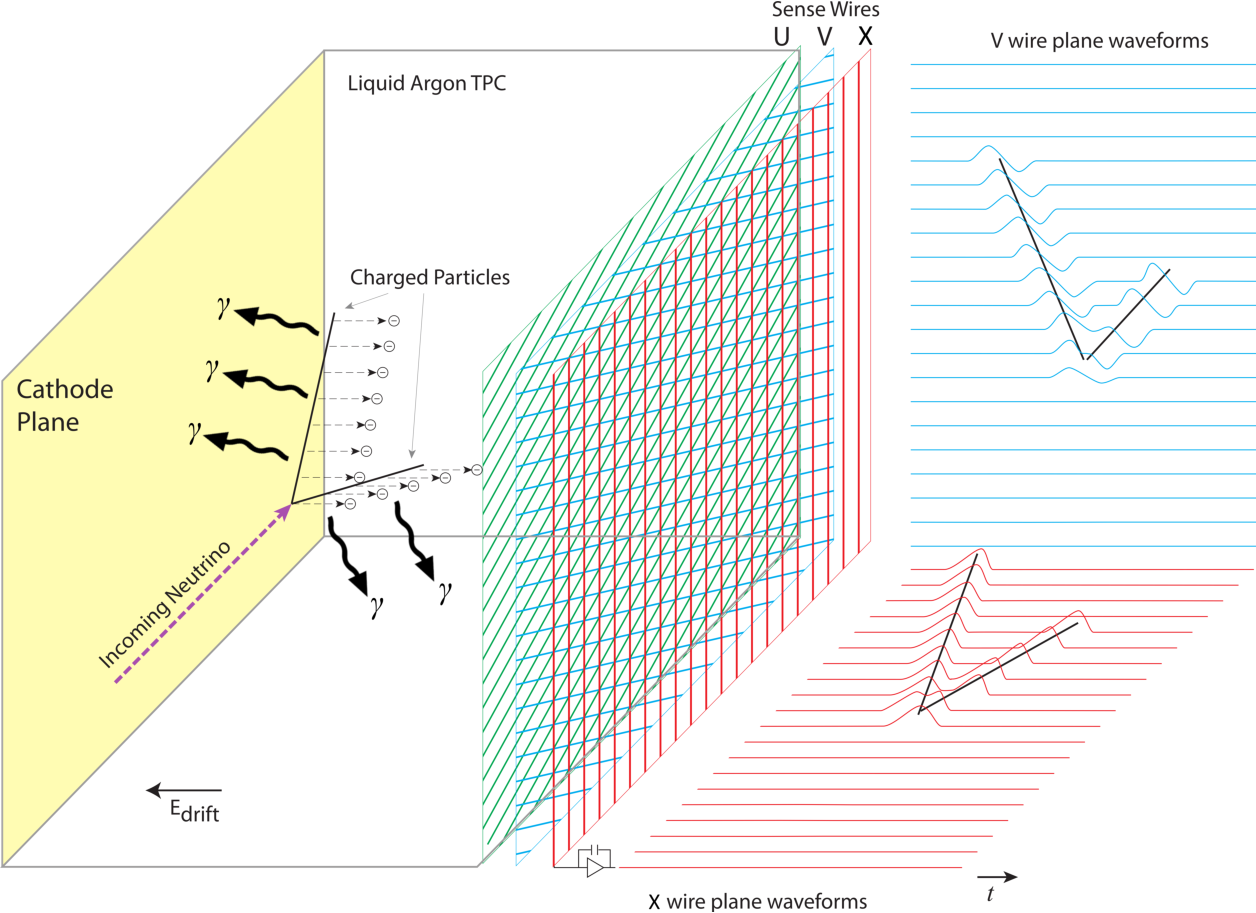
\includegraphics[width=\textwidth]{figures/LArTPC_Concept.pdf}

	\caption
	[LArTPC detection principal.]
	{LArTPC detection principal. Figure from \cite{Acciarri:2016smi}.}

	\label{fig:lartpc}

\end{figure}

The details of the charge readout and photon detection systems are specific to 
each detector, but broadly speaking LArTPC detectors can be split into two 
main categories: single--phase and dual--phase. In a single--phase detector the
drifting ionisation electrons remain in the liquid argon and the signals are 
typically read out on three anode wire planes. A dual--phase LArTPC contains an
additional region of gaseous argon in which a high electric field, known as the
extraction field, is applied to extract the ionisation from the liquid 
before it is amplified and collected on a pair of anode wire planes 
\cite{Abi:2020wmh}.

\bigskip

\protodune{} is one of two large scale prototypes for the DUNE far detector
modules, which focusses on the single--phase LArTPC technology. The DUNE far
detector modules feature a modular design in which each module is built up of a
number of identical components, \protodune{} was designed to prototype the
design of many of these components at a 1:1 scale, including the anode planes,
cathode plane, and photon detectors. The \protodune{} experiment has four 
primary goals, as outlined in the Technical Design Report \cite{Abi2017}:
\begin{itemize}
	\item Prototype the production and installation procedures for the
	single--phase far detector design.
	\item Validate the design from the perspective of basic detector performance;
	this can be achieved with cosmic-ray data. 
	\item Accumulate large samples of test-beam data to understand/calibrate the
	response of the detector to different particle species.
	\item Demonstrate the long-term operational stability of the detector as part
	of the risk mitigation program ahead of the construction of the first 10 kt
	far detector module.
\end{itemize}
As such, \protodune{} represents a significant milestone in the development of
the far detector for the DUNE experiment. Its successful operation, both in a 
test--beam and with cosmic rays, provides valuable data with which to understand
reconstruction and analysis of the data that will be collected by the DUNE far 
detector.

\section{The \protodune{} Detector} \label{sec:pdsp_detector}

The \protodune{} detector is located at the Neutrino Platform at CERN along the
H4 beamline. It is a single--phase LArTPC detector with a total liquid argon 
mass of 0.77 kt, making it the largest single--phase liquid argon TPC built to 
date. 

\subsection{The Cryostat}

\subsection{The Liquid Argon TPC}

\subsection{The Photon Detection System}

\subsection{The Cosmic Ray Taggers}

\subsection{The Data Acquisition System}


\section{The H4 Beam Line} \label{sec:h4}


\section{Cosmic Rays in ProtoDUNE--SP} \label{sec:pdsp_cosmic}


\section{ProtoDUNE--SP Simulation and Reconstruction} \label{sec:pdsp_sim_reco}

\subsection{Simulation}

\subsection{Reconstruction}

\section{ProtoDUNE--SP Online Monitoring System} \label{sec:pdsp_om}

